%Autor: Simon Walker
%Version: 1.0
%Datum: 02.12.2019
%Lizenz: CC BY-NC-SA

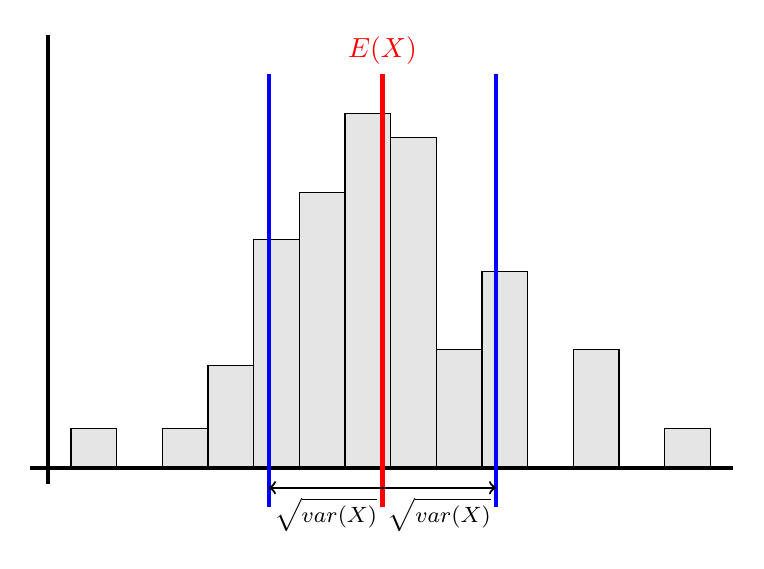
\begin{tikzpicture}[xscale=0.58, yscale=1]
	\def\values{{0.5, 0, 0.5, 1.3, 2.9, 3.5, 4.5, 4.2, 1.5, 2.5, 0, 1.5, 0, 0.5}}
	\def\EWert{7.32}
	\def\StAbw{2.49}
	
	%Histogramm werte
	\foreach \i in {0,1,...,13}
		\filldraw[draw=black, fill=gray!20] (\i+0.5, 0) rectangle (\i+1.5, \values[\i]);
	
	%Achsen
	\draw[ultra thick] (0,-0.2) -- (0,5.5);
	\draw[ultra thick] (-0.4, 0) -- (15,0);
	
	%Erwartungswert
	\draw[ultra thick, red] (\EWert,-0.5) -- (\EWert,5);
	\node[above, red] at (\EWert,5){$E(X)$};
	
	%Varianz
	\draw[ultra thick, blue] (\EWert-\StAbw,-0.5) -- (\EWert-\StAbw,5);
	\draw[ultra thick, blue] (\EWert+\StAbw,-0.5) -- (\EWert+\StAbw,5);
	\draw [<->, thick] (\EWert-\StAbw, -0.25) -- (\EWert+\StAbw, -0.25);
	\node[below] at ({\EWert-(\StAbw/2)},-0.25){\footnotesize$\sqrt{var(X)}$};
	\node[below] at ({\EWert+(\StAbw/2)},-0.25){\footnotesize$\sqrt{var(X)}$};
	
		
%	\newcommand{\HelpCords}[4]{
%		\draw [help lines] (#1,#2) grid (#3,#4);
%		\foreach \i in {#1,..., #3}
%		\node [below] at (\i,#2) {$\i$};
%		\foreach \i in {#2,..., #4}
%		\node [left] at (#1,\i) {$\i$};
%	}
%	\HelpCords{0}{0}{15}{5.5}
\end{tikzpicture}
